\documentclass{article}
\usepackage[utf8]{inputenc}

% Standard packages that I use for math documents.
\usepackage[margin=0.75in]{geometry}
\usepackage{enumerate}
\usepackage{amsmath}
\usepackage{amsfonts} 
\usepackage{amssymb}
\usepackage{amsthm}
\usepackage{mathtools}
\usepackage{float}
\usepackage{array}
\usepackage{makecell}
\usepackage{commath}
\usepackage{easybmat} % for block matrices
\usepackage{parskip}
% Document-specific packages
\usepackage{xcolor, soul} % for highlights
\sethlcolor{yellow}

% Standard settings I use for nice formatting.
\setlength\parindent{0pt}
\DeclarePairedDelimiter{\ceil}{\lceil}{\rceil}
\renewcommand\theadalign{bc}
\renewcommand\theadfont{\bfseries}
\renewcommand\theadgape{\Gape[4pt]}
\renewcommand\cellgape{\Gape[4pt]}

% Standard definitions of macros I use regularly.
\newcommand{\N}{\mathbb{N}}
\newcommand{\Z}{\mathbb{Z}}
\newcommand{\Q}{\mathbb{Q}}
\newcommand{\C}{\mathbb{C}}
\newcommand{\R}{\mathbb{R}}
\newcommand{\F}{\mathbb{F}}
\newtheorem{theorem}{Theorem}
\newtheorem{proposition}{Proposition}[section]
\newtheorem{conjecture}{Conjecture}[section]
\newtheorem{corollary}{Corollary}[theorem]
\newtheorem{definition}{Definition}[section]
\newtheorem{lemma}[theorem]{Lemma}
\newtheorem*{remark}{Remark}
\newcommand{\cdotscalar}{\;\widetilde{\cdot}\;}
\newcommand{\vectorplus}{\;\widetilde{+}\;}
\newcommand{\Span}{\text{Span}}
\newcommand{\Null}{\text{Null}}
\newcommand{\Range}{\text{Range}}
\newcommand{\D}{\frac{d}{\dif x}}
\renewcommand{\epsilon}{\varepsilon}
\newcommand{\Or}{\mbox{ OR }}
\renewcommand{\And}{\mbox{ AND }}
\newcommand{\Not}{\mbox{NOT }}
\newcommand{\Iff}{\mbox{ IFF }}
\newcommand{\Width}{\textup{width}}
\newcommand{\Mesh}{\textup{mesh}}
\newcommand{\Int}{\textup{Int}}
\newcommand{\Ext}{\textup{Ext}}
\newcommand{\Bd}{\textup{Bd}}
\newcommand{\Supp}{\textup{Support}}
\newcommand{\sgn}{\textup{sgn}}
\newcommand{\loss}{\textup{loss}}
\newcommand{\insamplegeqx}{\textup{\texttt{insample$\geq$x}}}
\newcommand{\insampleltx}{\textup{\texttt{insample$<$x}}}
\newcommand{\insample}{\textup{\texttt{insample}}}
\newcommand\widebar[1]{\mathop{\overline{#1}}}
\newcommand*\closure[1]{\widebar{#1}}
\newcommand\Ball[2]{U(#1; #2)}

\newcommand{\1}{\langle 1 \rangle}
\newcommand{\2}{\langle 2 \rangle}
\renewcommand*\abstractname{Summary}

% End of preamble.  

\begin{document}

\title{Optimizing shift-coupling proofs of privacy for DiPA}
\date{Summer Research: May -- August 2023}
\author{Vishnu Nittoor}

\maketitle

\begin{abstract}
    This document is a summary of the work done this summer on finding tight privacy bounds for DiPA using probabilistic couplings. We restrict ourselves to shift-couplings, which are couplings on the noise of neighbouring inputs on transitions. We find necessary and sufficient conditions on shift-couplings to show $\epsilon$-differential privacy, and show that finding a tight shift-coupling proof of privacy can be formulated as an optimization problem. We show that tight shift-coupling proofs must necessarily depend on the differences between neighbouring inputs, and the paths taken by the automaton on those inputs. 
    
    We present the notion of a segment, which allows us to optimize over finitely many families of paths. Although the search for a tight proof is a convex maximization problem, a relaxation can be formulated as linear programs over segment sequences. We bound the cost of a tight proof of privacy in terms of the cost of the tight relaxated shift-coupling proof, and show that differential privacy can be decided in linear-time for DiPA using the model of shift-couplings. An open problem is whether there exist privacy bounds for DiPA that cannot be shown using shift-couplings.
\end{abstract}
\tableofcontents

\newpage

% \section{Some notes from which to expand this document}

% \begin{enumerate}
%     \item An overview of coupling proofs of privacy
%     \item A tight shift-coupling proof of privacy (segment free)
%     \begin{enumerate}
%         \item What are the connecting constraints, and why are they there?
%         \item Proofs have to depend on $\Delta$!
%         \item Proofs have to depend on sequences of segments! 
%     \end{enumerate}
%     \item Simplifying the problem above in various ways: 
%     \begin{enumerate}
%         \item Separability and the introduction of segments
%         \item Only inter-segment transitions matter! 
%         \begin{itemize}
%             \item Given $\Delta$, the $\gamma$ values on inter-segment transitions are easily determined. 
%             \item The $\Delta$ values on the inter-segment transitions can be determined. 
%         \end{itemize}
%     \end{enumerate}
%     \item Solving the problem.
%     \begin{enumerate}
%         \item Hardness (incomplete)!!!
%         \item Solving the easier version, where proofs don't depend on $\Delta$.
%         \item Showing that they are bounded within $n$ of each other. 
%         \begin{align*}
%             \exists \text{ finite DP bound } &\iff \text{ hard system admits a feasible solution }
%         \end{align*}
%     \end{enumerate}
% \end{enumerate}

% \subsection{DiPA}

% Insert definition for DiPA here. 

% \subsection{Probability}

% \begin{definition}
%     The probability $\Pr(\rho | X)$ of a path $\rho = q_0 \to q_1 \to \dots \to q_m$ given an input $X = \langle a_1 , \dots, a_m \rangle$ is defined recursively as the probability that all transitions in $\rho$ are traversed in sequence given the input $X$ starting at state $q_0$.
% \end{definition}

% \begin{definition}
%     Let $\mathcal{A}$ be a DiPA, and $s \in seg(\mathcal{A})$ be a segment. The \textbf{privacy loss} $\loss(s)$ of a segment $s \in seg(\mathcal{A})$ is defined as 

%     \[\loss(s) = \sup_{\rho \in segF(s)}\sup_{X' \sim X} \left(\frac{Pr(\rho | X)}{P(\rho | X')} \right) \]

%     where $X$ and $X'$ vary over all pairs of neighbouring datasets. 
% \end{definition}

% \begin{definition}
%     Let $f_\epsilon(x)$ be the probability density function of a random variable $X$ with $X \sim Lap(0, 1/\epsilon)$. 

%     \[f_\epsilon(x) = \frac{\epsilon}{2} \exp(-\epsilon |x|)\]
% \end{definition}

% \begin{definition}
%     Let $F_\epsilon(x)$ be the cumulative distribution function of a random variable $X$ with $X \sim Lap(0, 1/\epsilon)$.

%     \[F_\epsilon(x) = P(X \leq x) = \begin{cases}
%         \frac{1}{2} \exp(\epsilon x) & x < 0 \\
%         1 - \frac{1}{2} \exp(-\epsilon x) & x \geq 0
%     \end{cases}\]
% \end{definition}

\section{Coupling proofs of privacy}

In order to set up shift-coupling proofs of privacy, we first need to define the notion of a coupling proof of privacy. 

\begin{definition}
    Let $\mathcal{A}$ be a randomized mechanism taking outputs in $B$. A \textbf{coupling proof of privacy} with cost $\epsilon$ for $\mathcal{A}$ constructs for every two adjacent inputs $X \1 \sim X \2$ and output $b \in B$ of $\mathcal{A}$ the coupling 

    \[\mathcal{A}(X \1) \Phi_b^{\#(\epsilon, 0)} A(X \2)\]

    where 

    \[\Phi_{b} = \{(x_1, x_2) \in B \times B : x_1 = b \implies x_2 = b\}\]
\end{definition}

\begin{proposition}
    A randomized mechanism $\mathcal{A}$ is $\epsilon$-differentially private if there exists a coupling proof of privacy for $\mathcal{A}$ with cost $\epsilon$.
\end{proposition}

\begin{proof}
    From "Proving Differential Privacy via Probabilistic Couplings" by Barthe et al. 
\end{proof}

\section{Shift-coupling proofs of privacy}

Shift-coupling proofs of privacy attempt to couple the neighbouring noised inputs read by a DiPA $\mathcal{A}$ on $X \1 \sim X \2$ using shifts in order to construct a coupling proof of privacy. In order to do this, we need to understand the correspondence between paths and outputs in a DiPA.

Let $path_{\mathcal{A}}(X)$ be a random variable representing the path taken by $\mathcal{A}$ on $X$, and $output_{\mathcal{A}}(X)$ be a random variable representing the output produced by $\mathcal{A}$ on $X$.

\begin{proposition}
    \label{prop:output_determinism}
    Let $\mathcal{A}$ be a DiPA, and $X \1 \sim X \2$ be two neighbouring inputs. We have 
    \begin{align*}
        path_{\mathcal{A}}(X \1) = path_{\mathcal{A}}(X \2) \text{ with same real-valued outputs} \iff output_{\mathcal{A}}(X \1) = output_{\mathcal{A}}(X \2)
    \end{align*}
    and 
    \begin{align*}
        path_{\mathcal{A}}(X \1) \Psi_\rho path_{\mathcal{A}}(X \2) \text{ with same real-valued outputs} \iff \forall o \in [o]_\rho : output_{\mathcal{A}}(X \1) \Phi_o output_{\mathcal{A}}(X \2)
    \end{align*}
    where $[o]_\rho$ is the class of all possible outputs that can be produced by the path $\rho$.
\end{proposition}

\begin{proof}
    This directly follows from the output determinism conditions in DiPA. 
\end{proof}

% Shift-couplings are a technique that relate every path taken by $\mathcal{A}$ on $X$ and $X'$ by a probabilistic coupling, from which we can relate all outputs produced by $\mathcal{A}$ on that path. We wish to construct the coupling

\begin{proposition}
    \label{prop:output_coupling}
    If we have for all $X \1 \sim X \2$ and paths $\rho$ taken by $\mathcal{A}$ that 
    \begin{align*}
        output_{\mathcal{A}}(X \1) \Psi_{\rho}^{\#(\epsilon, 0)} output_{\mathcal{A}}(X \2) \\[1em]
        \Psi_{\rho} = \{(o_1, o_2) \in B \times B : o_1 \in [o]_\rho \implies o_1 = o_2\}
    \end{align*}

    then $\mathcal{A}$ is $(\epsilon, 0)$-differentially private.
\end{proposition}

\begin{proof}
    For any output $o \in B$, find the path $\rho$ for which $o \in [o]_\rho$. Then we can construct the coupling

    \[output_{\mathcal{A}}(X \1) \Phi_o^{\#} output_{\mathcal{A}}(X \2)\]

    where 

    \[\Phi_o = \{(o_1, o_2) \in B \times B : o_1 = o \implies o_2 = o\}\]

    which shows $(\epsilon, 0)$-privacy. 
\end{proof}

The goal of shift-coupling proofs of privacy is to construct the lifting in Proposition \ref{prop:output_coupling} by the relation $\Psi_\rho$. This is because working with paths is more amenable to shift-couplings than working with outputs.

\begin{definition}
    Let  $X = \langle a_1, \dots, a_m \rangle$ be an input, and $\rho = q_0 \to q_1 \to \dots \to q_m$ be a path taken by DiPA $\mathcal{A}$ on $X$. Define $\tilde{a_i}$ to be the value of $\insample$ on the $i$th transition in $\rho$ on input $X$.
\end{definition}

A shift-coupling proof of privacy attempts to construct the couplings in Proposition \ref{prop:output_coupling}  by constructing the couplings for $X \1 = \langle a_1 \1, \dots, a_m \1 \rangle$ and $X \2 = \langle a_1 \2, \dots, a_m \2 \rangle$ for all $a_i \1, a_i \2 \in [-1, 1]$. Let us use the notation \[\tilde{a} \1 + \boldsymbol{\gamma} = \tilde{a} \2\] to denote the couplings \begin{align*}
    \tilde{a}_i \1 + \gamma_i =^{\#} \tilde{a}_i \2 \qquad \forall i 
\end{align*}

We call $\boldsymbol{\gamma}$ an assignment of shifts.

\begin{definition}
    
    Given a fixed path, we say that an assignment of shifts $\boldsymbol{\gamma} = \{\gamma_i\}$ is \textbf{path-valid} if
    
    \[(\tilde{a} \1 + \gamma = \tilde{a} \2) \implies \big(path_{\mathcal{A}}(X \1) = \rho \implies path_{\mathcal{A}}(X \2) = \rho \big)\]
    
    \end{definition}
    
    \begin{definition}
        Given a fixed path, we say that an assignment of shifts $\boldsymbol{\gamma} = \{\gamma_i\}$ is \textbf{valid} if
    
        \[(\tilde{a} \1 + \gamma = \tilde{a} \2) \implies \big(output_{\mathcal{A}}(X \1) \Psi_\rho output_{\mathcal{A}}(X \2) \big)\]
    
        where $\Psi_\rho$ is the relation on outputs defined by
    
        \[\Psi_\rho = \{(o_1, o_2) \in B \times B : o_1 \in [o]_\rho \implies o_1 = o_2\}\]
    \end{definition}


    \begin{definition}
        Given a DiPA $\mathcal{A}$, a \textbf{shift-coupling proof of privacy} for $\mathcal{A}$ is a map 
    
        \begin{align*}
            \Gamma: paths(\mathcal{A}) &\to ([-1, 1]^{|\rho|} \to [-1, 1]^{|\rho|})\\
            \rho &\mapsto (\Delta \mapsto \{\gamma_i\})
        \end{align*}
    
        such that for all $\rho \in paths(\mathcal{A})$ and all $\Delta \in [-1, 1]^{|\rho|}$, we have that $\{\gamma_i\}$ is valid for $\rho$.
    \end{definition}

    We choose $\gamma \in [-1, 1]$ as any choice of $\gamma \in \R$ can be projected to $[-1, 1]$ to construct a valid shift-coupling proof of privacy without increasing 'cost', as defined below.

\subsection{Constraints} 
We now wish to find necessary and sufficient conditions on $\boldsymbol{\gamma}$ that ensure that it is valid.

\begin{definition}
    Let $\rho = q_0 \to q_1 \to \dots \to q_m$ be a path, and let $i \in \{1, \dots, m\}$. Define $at(i)$ to be the largest index $a(i) < i$ such that $\rho[a(i)] \to \rho[a(i) + 1]$ is an assignment transition.  
\end{definition}

Note that such an index must exist due to the initialization condition on DiPA. 

\begin{proposition}
    Given $\rho = q_0 \to q_1 \to \dots \to q_m$, an assignment of shifts $\boldsymbol{\gamma} = \{\gamma_i\}$ is path-valid if and only if it satisfies the following constraints for all $i \in \{0, \dots, m - 1\}$:

    \begin{align}
        \gamma_i \leq \gamma_{at(i)} \qquad &\text{if } t_i \text{ has guard } < \\
        \gamma_i \geq \gamma_{at(i)} \qquad &\text{if } t_i \text{ has guard } \geq 
    \end{align}

    where $t_i = q_i \to q_{i + 1}$ is the $i$th transition in $\rho$.
\end{proposition}

\begin{proof}
    (Constraints $\implies$ path-valid) Suppose that the above constraints hold. We will show that $\{\gamma_i\}$ is path-valid using induction on $m = |\rho|$. Construct the couplings $\tilde{a_i} \1 + \gamma_i (=)^{(\epsilon_i, 0)} \tilde{a_i} \2$ for all $i \in \{0, \dots, m - 1\}$. 

    For a base case, assume $m = 1$. Then $\rho$ consists of an assignment transition $t_0$ with \texttt{true} guard (initialization condition). The constraints are trivially satisfied, and we have that $path_{\mathcal{A}}(X \1 ) \Psi_\rho^{(0, 0)} path_{\mathcal{A}}(X \2)$.

    Assume that the constraints hold for all paths of length $m$. Let $\rho = q_0 \to q_1 \to \dots \to q_{m} \to q_{m + 1}$. We will show that $\{\gamma_i\}$ is path-valid for $\rho$. First, by the path-validity of $\{\gamma_i\}_{i = 0}^{m - 1}$ for $\rho[0:m]$ by the inductive hypothesis, we have that \[path_{\mathcal{A}}(X \1) \Psi_{\rho[0:m]} path_{\mathcal{A}}(X \2)\] 
    
    by the inductive hypothesis. Now, assume $path_{\mathcal{A}}(X \1) = \rho$. We have $path_{\mathcal{A}}(X \2)[0:m] = \rho[0:m]$. Consider the last transition $t_{m}$ in $\rho$. Since $path_{\mathcal{A}}(X \1) = \rho$, we know that $t_m$ is traversed by $A$ on $X \1$.

    \begin{itemize}
        \item If $t_{m}$ has guard \texttt{true}, then we trivially have that $path_{\mathcal{A}}(X \2) = \rho$.
        \item If $t_{m}$ has guard $<$, we have from the constraints that $\gamma_{m} \leq \gamma_{at(m)}$. The value of the state variable $x \langle 1 \rangle$ is 
        
        \[x \1 = \tilde{a}_{at(m)} \1 \]

        and since $t_m$ is traversed by $A$ on $X \1$, we have 

        \begin{align*}
            \tilde{a}_{m} \1 &< \tilde{a}_{at(m)} \1\\
            \tilde{a}_{m} \2 - \gamma_m &< \tilde{a}_{at(m)} \2 - \gamma_{at(m)}\\
            \tilde{a}_{m} \2 &< \tilde{a}_{at(m)} \2 - (\gamma_{at(m)} - \gamma_{m}) < \tilde{a}_{at(m)} \2\\
        \end{align*}

        showing that $\tilde{a}_{m} \2$ satisfies the guard of $t_m$. Thus, $path_{\mathcal{A}}(X \2) = \rho$.
        \item If $t_{m}$ has guard $\geq$, a similar argument as above shows that $path_{\mathcal{A}}(X \2) = \rho$.
    \end{itemize}

    Thus, assuming that $a \1 + \gamma = a \2$, we have shown that $path_{\mathcal{A}}(X \1) = \rho \implies path_{\mathcal{A}}(X \2) = \rho$, which shows $path_{\mathcal{A}}(X \1) \Psi_\rho path_{\mathcal{A}}(X \2)$, and so $\{\gamma_i\}$ is path-valid.

    (Path-valid $\implies$ constraints) Suppose that $\{\gamma_i\}$ is path-valid. Let $i \in \{0, \dots, m - 1\}$. We will show that the constraints hold for $i$. 

    We will run the argument above in reverse. Again, we use induction on the length $m = |\rho|$. For a base case, assume $m = 1$, and so $\rho$ consists of an assignment transition $t_0$ with \texttt{true} guard. The constraints are trivially satisfied, since there are none. 

    Assume that the constraints hold for all path-valid shift assignments on paths of length $m$, and let $\rho = q_0 \to q_1 \to \dots \to q_{m} \to q_{m + 1}$. Since $\{\gamma_i\}$ is path-valid for $\rho$, we have that $a \1 + \gamma = a \2 \implies path_{\mathcal{A}}(X \1) \Psi_\rho path_{\mathcal{A}}(X \2)$. Also, we have that $\{\gamma_i\}_{i = 0}^{m - 1}$ is path-valid for $\rho[0:m]$, and that constraints on transitions $t_i \in \rho[0:m]$ hold. 

    We will now show that the constraints on $t_{m}$ hold by cases on the guard of $t_{m}$.

    \begin{itemize}
        \item If $t_{m}$ has guard \texttt{true}, then there is no constraint on $\gamma_{m}$, and so the constraints hold.
        \item If $t_{m}$ has guard $<$, the constraint to be shown is $\gamma_m \leq \gamma_{at(m)}$. Recall that we have $a \1 + \gamma = a \2 \implies path_{\mathcal{A}}(X \1) \Psi_\rho path_{\mathcal{A}}(X \2)$, showing that $t_m$ being traversed by $A$ on $X \1$ leads $t_m$ to be traversed by $A$ on $X \2$. Thus, we have 
        
        \begin{align*}
            \tilde{a}_m \1 < \tilde{a}_{at(m)} \1 &\implies \tilde{a}_m \2 < \tilde{a}_{at(m)} \2\\
             &\iff \tilde{a}_m \1 + \gamma_m < \tilde{a}_{at(m)} \1 + \gamma_{at(m)}\\
             &\iff \tilde{a}_m \1 < \tilde{a}_{at(m)} \1 + (\gamma_{at(m)} - \gamma_m)\\
        \end{align*}

        which is true if and only if $\gamma_m \leq \gamma_{at(m)}$. Thus, the constraint holds.
        \item A symmetric argument shows that the constraint holds if $t_{m}$ has guard $\geq$.
    \end{itemize}

    Thus, the given constraints on $\gamma$ hold if and only if it is path-valid for $\rho$.
\end{proof}

\begin{proposition}
    A shift assignment $\boldsymbol{\gamma} = \{\gamma_i\}$ is valid for $\rho$ if and only if it is path-valid for $\rho$ and satisfies the following output determinism constraint:
    \begin{align*}
        \gamma_i = 0 \qquad &\text{if } t_i \text{ outputs } \insample \text{ or } \insample'
    \end{align*}
\end{proposition}

\begin{proof}
    To obtain path validity and the output determinism constraint from validity and vice versa, one applies Proposition \ref{prop:output_determinism}.
\end{proof}

\subsection{The cost of a shift-coupling}

\begin{proposition}
    Consider a transition $t_i = q_{i} \to q_{i + 1}$ which is traversed independently by $A$ on input $a_i \1$ and $a_i \2$. Let $\Delta_i = a_i \2 - a_i \1$. Let $q_i$ draw from the distribution $Lap(0, \epsilon_i)$ to noise \texttt{insample}. The cost of the coupling 

    \[\tilde{a_i} \1 + \gamma_i (=)^{(c_i, 0)} \tilde{a_i} \2\]

    is given by \[c_i = |\Delta_i - \gamma_i| \epsilon_i \]
\end{proposition} 

\begin{proof}
    This is seen from coupling construction rules.
\end{proof}

\begin{definition}
    Given a path $\rho$ and input differences $\Delta$, we define the $\rho$-$\Delta$-\textbf{cost} of the shifts $\gamma = \{\gamma_i\}$ to be

    \[\rho{\text -}\Delta{\text -}cost(\gamma) = \sum_{i = 0}^{|\rho| - 1} |\Delta_i - \gamma_i| \epsilon_i\]
\end{definition}

\begin{definition}
    Given a path $\rho$ and a shift-coupling proof of privacy $\Gamma$ define the $\rho$-\textbf{cost} of $\Gamma$

    \[\rho{\text -}cost(\Gamma) = \sup_{\Delta \in [-1, 1]^{|\rho|}} \rho{\text -}\Delta{\text -}cost(\Gamma(\rho, \Delta))\]
\end{definition}

\begin{definition}
    Given a shift-coupling proof of privacy $\Gamma$, we define the privacy cost of $\Gamma$ to be

    \[cost(\Gamma) = \sup_{\rho \in paths(\mathcal{A})} \rho\text{-}cost(\Gamma)\]
\end{definition}

\subsection{Tight proofs of privacy}

\begin{theorem}
    Let $\mathcal{A}$ be a DiPA, and $\Gamma$ be a shift-coupling proof of privacy for $\mathcal{A}$ with finite cost $\epsilon = cost(\Gamma)$. Then, $\mathcal{A}$ is $(\epsilon, 0)$-differentially private.
\end{theorem}

\begin{proof}
    This is a direct consequence of output validity. 
\end{proof}

Since the total validity constraints on $\{\gamma_i\}$ does not depend on $X \1$ and $X \2$, one might be tempted to produce a proof of privacy by choosing $\gamma_i$ to be the same for all $X \1$ and $X \2$, given a path $\rho$. Although this is possible, this does not in general produce a tight proof of privacy.

\begin{proposition}
    \label{prop:proofs_must_regard_input_differences}
    \textbf{(A tight proof must regard input differences)} There exists a family of DiPA $\mathcal{F}$ and for $\mathcal{A} \in \mathcal{F}$, a shift-coupling proof $\Gamma^*: paths(\mathcal{A}) \to ([-1, 1]^{\rho} \to [-1, 1]^{|\rho|})$ such that for all assignments $\Pi: paths(\mathcal{A}) \to [-1, 1]^{\rho}$ of paths to shifts, we have 

    \[cost(\Gamma^*) < cost(\Pi)\]
\end{proposition}

\begin{proof}
    The construction is a DiPA with a path with one assignment transition, and the same number of $<$ and $\geq$ transitions.
\end{proof}

When constructing a shift-coupling proof of privacy, we are actually choosing a shift for each transition. Is it reasonable to ignore paths, and just choose a shift for each transition? The answer is no, as the following proposition shows.

\begin{proposition}
    \label{prop:proofs_must_regard_paths}
    \textbf{(A tight proof must regard paths)} There exists a family of DiPA $\mathcal{F}$ and for $\mathcal{A} \in \mathcal{F}$, a shift-coupling proof $\Gamma^*: paths(\mathcal{A}) \to ([-1, 1]^{\rho} \to [-1, 1]^{|\rho|})$ such that for all assignments $\Pi: E \to ([-1, 1]^{\rho} \to [-1, 1]^{\rho})$ of transitions and differences to shifts, we have

    \[cost(\Gamma^*) < cost(\Pi)\]
\end{proposition}

\begin{proof}
    In the construction, we have a DiPA for which there are two constraints on three assignment transitions, but also the assignment transition followed by $\gamma_1$ has a cycle of $<$ transitions before reaching the $\gamma_3$ assignment transition. For finite cost, this forces $\gamma_1 = 1$.
    \begin{align*}
        \gamma_1 &\leq \gamma_3 \\
        \gamma_2 &\leq \gamma_3
    \end{align*}
    Then satisfying this constraint system also requires $\gamma_3 = 1$, which forces a high cost on paths that pass through the $\gamma_2$ and $\gamma_3$ transitions. We can achieve a lower maximum cost by assigning shifts independently to paths. 
\end{proof}

\section{The search for a tight proof as an optimization problem}

\subsection{Stating the problem abstractly}

Now that we have a characterization of shift-coupling proofs of privacy, the problem of finding a tight proof of privacy can be formulated as finding, given $\rho$ and $\Delta$,

\begin{align*}
    \inf_{\Gamma} cost(\Gamma) &= \inf_{\Gamma} \sup_{\rho} \sup_{\Delta} \rho\text{-}\Delta\text{-}cost(\Gamma(\rho, \Delta)) \\
\end{align*}

which is characterized by $\Gamma^*$ such that for any shift-coupling proof $\Gamma$, we have

\[\sup_{\rho} \sup_{\Delta} \rho\text{-}\Delta\text{-}cost(\Gamma^*(\rho, \Delta)) \leq \sup_{\rho} \sup_{\Delta} \rho\text{-}\Delta\text{-}cost(\Gamma(\rho, \Delta))\]


One such $\Gamma^*$ is the shift-coupling proof that chooses \[\Gamma^*(\rho, \Delta) = \inf_{\gamma \in [-1, 1]^{|\rho|}} \rho\text{-}\Delta\text{-}cost(\Delta, \gamma)\]

which is the shift-coupling proof that chooses the optimal shift for each input difference and path independently. We will now direct our focus to computing $\Gamma^*$ given an automaton $\mathcal{A}$.

\subsection{Simplifying the problem with fixed $\rho, \Delta$}

\begin{proposition}
    \label{prop:gammas_non_assignment}
    Let $\rho, \Delta$ be given, and let 
    
    \[\gamma_i^* = \arg \inf_{\gamma \in [-1, 1]^{|\rho|}} \rho\text{-}\Delta\text{-}cost (\gamma)\]
    
    For non-assignment transitions $t_i \in \rho$, we have that 

    \begin{align*}
        \gamma_i^* &= \min(\Delta_i, \gamma_{at(i)}) \qquad \text{if } t_i \text{ has guard } < \\
        \gamma_i^* &= \max(\Delta_i, \gamma_{at(i)}) \qquad \text{if } t_i \text{ has guard } \geq \\
    \end{align*}
\end{proposition}

\begin{proof}
    Missing, but I have notes for it. The proof comes from noting that shifts non-assignment transitions have only one linear constraint, and so we can solve for them optimally in terms of the shift on the previous assignment transition. 
\end{proof}

% \begin{corollary}
%     Let $\rho$ be given, and let $t_i$ and $t_j$ be two instances in which the same non-assignment transition is traversed in $\rho$. If $at(i) = at(j)$, then $\gamma_i = \gamma_j$. 
% \end{corollary}

% \begin{proposition}
%     If there exists a path $\rho$ which has the same assignment transition traversed twice, then $\mathcal{A}$ is not $\epsilon$-differentially private for any $\epsilon$.
% \end{proposition}

% \begin{corollary}
%     Let $\rho$ be given with each assignment transition traversed at most once. Then, if two instances $t_i$, $t_j$ of the same non-assignment transition are traversed in $\rho$, they must have $at(i) = at(j)$.
% \end{corollary}

% The above corollaries are important as they show that we can roll-up traversals of a non-assignment transition on a cycle into a single traversal, and so only need to consider one shift.

% \begin{definition}
%     Let $\rho$ be a path. Define the function $acyclic: P \to P$ such that $acyclic(\rho)$ is the path obtained by removing all cycles in $\rho$. (TODO: Perhaps elaborate using Sky's definition of acyclic)
% \end{definition}

% \begin{definition}
%     Let $paths(\mathcal{A})_{eq}$ be the set of equivalence classes of paths, where $\rho, \rho' \in paths(\mathcal{A})$ are equivalent if $acyclic(\rho) = acyclic(\rho')$.
% \end{definition}

\subsection{Simplifying the problem with fixed $\rho$}

\begin{proposition}
    \label{prop:deltas_non_assignment}
    Let $\rho$ be given. Let \[\Delta^* = \arg \sup_{\Delta \in [-1, 1]^{|\rho|}} \inf_{\gamma \in [-1, 1]^{|\rho|}} \rho\text{-}\Delta\text{-}cost (\gamma)\]
    
    For non-assignment transitions $t_i \in \rho$, we have that 

    \begin{align*}
        \Delta_i^* = \begin{cases}
            1 & \text{if } t_i \text{ has guard } < \\
            -1 & \text{if } t_i \text{ has guard } \geq \\
        \end{cases}
    \end{align*}
\end{proposition}

\begin{proof}
    Missing, but I have notes for it. The proof goes by showing that the solution to the inner problem is at least as much as the solution to the inner problem with $\Delta_i = 1$ or $\Delta_i = -1$ respectively.
\end{proof}

\begin{corollary}
    \label{cor:non_assignment_solved}
    Let $\rho$ be given. Let \[\Delta^* = \arg \sup_{\Delta \in [-1, 1]^{|\rho|}} \inf_{\gamma \in [-1, 1]^{|\rho|}} \rho\text{-}\Delta\text{-}cost(\gamma)\]
    \[\gamma^* = \arg \inf_{\gamma \in [-1, 1]^{|\rho|}} \rho\text{-}\Delta\text{-}cost(\gamma)\]
    As a consequence of Propositions \ref{prop:gammas_non_assignment} and \ref{prop:deltas_non_assignment}, if $t_i \in \rho$ is a non-assignment transition, then \[\gamma_i^* = 
    \gamma^*_{at(i)}\].

    % Proof: 
    % \begin{cases}
    %     \min(\gamma^*_{at(i)}, \Delta^*_i) & \text{if } t_i \text{ has guard } < \\
    %     \max(\gamma^*_{at(i)}, \Delta^*_i) & \text{if } t_i \text{ has guard } \geq \\
    %     \end{cases} = \begin{cases}
    %         \min(\gamma^*_{at(i)}, 1) & \text{if } t_i \text{ has guard } <  \\
    %         \max(\gamma^*_{at(i)}, -1) & \text{if } t_i \text{ has guard } \geq \\
    %         \end{cases}
\end{corollary}

The corollary above is important: it reveals that the only transitions that matter are assignment transitions!

\subsubsection{Identifying segments}

Corollary \ref{cor:non_assignment_solved} allows us to formulate the problem of finding cost-minimal shifts $\gamma$ over maximal input differences $\Delta \in [-1, 1]^{|\rho|}$ given $\rho$ to the problem of finding $\gamma$ and $\Delta$ for only the assignment transitions in $\rho$. This motivates the definition of a \textit{segment} -- a way of identifying paths in order to consider finitely many classes of paths.

\begin{definition}
    Consider a DiPA $\mathcal{A}$. Let $q_i, q_j \in Q$ be such that there is a path $\rho = a_1 \to \dots \to a_m$ such that:

    \begin{itemize}
        \item $a_1 = q_i$ and $a_m = q_j$
        \item $a_1 \to a_2$ is the only assignment transition in $\rho$
        \item There exists an assignment transition out of $q_j$ or it is a terminal state
    \end{itemize}

    Then we define $seg(q_i, q_j)$ to be the set of all paths from $q_i$ to $q_j$ that are acyclic with their first transition being their only assignment transition. We call such a path $s \in seg(q_i, q_j)$ a \textbf{segment}. 
\end{definition}

\begin{definition}
    Given a segment $s \in seg(q_i, q_j)$, define the \textbf{segment family} $segF(s)$ to be the set of all paths $\rho$ from $q_i$ to $q_j$ such that the only assignment transition in $\rho$ is from $q_i$ and $acyclic(\rho) = s$.
\end{definition}

\begin{proposition}
    \label{prop:segmenting}
    Consider a path $\rho$ with assignment transitions from states $a_0, a_2, \dots, a_{n - 1}$, and terminal state $a_n$. There exists a unique sequence of segments $s_1 \hookrightarrow s_2 \hookrightarrow \dots \hookrightarrow s_n$ such we can write $\rho = \rho_1 \circ \rho_2 \circ \dots \circ \rho_n$ where $\rho_i \in segF(s_i)$ for all $i \in \{1, \dots, n\}$.
\end{proposition} 

\begin{proof}
    This is straightforward.
\end{proof}

Since we know from Corollary \ref{cor:non_assignment_solved} that shifts on a segment are equal to the shift on the assignment transition of the segment, we need only consider pairs of $\Delta, \gamma \in \R$ for the assignment transition of the segment. From this, we can deduce the $\gamma$-minimal cost with respect to maximal $\Delta$ for any path in the segment family.

\begin{definition}
    Let $s \in seg(q_i, q_j)$ be a segment, and let $\Delta, \gamma \in \R$ be the input difference and shift for the assignment transition of $s$. Define the \textbf{$s$-segment cost} of $\Delta$ and $\gamma$ to be

    \[s\text{-}segcost(\Delta, \gamma) = \sup_{\rho \in segF(s)} \rho\text{-}cost(\Gamma) \]

    where $\Gamma$ is a coupling strategy that chooses shift $\gamma$ for all transitions in $s$ given maximal non-assignment transition input differences with assignment input difference $\Delta$.
\end{definition}

The above is well-defined since the maximizing input differences for non-assignment transitions are determined independently of $\Delta$, and the optimal shifts on those transitions with respect to the differences depend only on $\gamma$. Now, we can begin to formulate finding optimal $\Delta$ and $\gamma$ for a path $\rho$ as an optimization problem over segments.

\begin{proposition}
    If a segment $s \in seg(q_i, q_j)$ has a cycle with a transition with guard $<$, then for $\Delta, \gamma \in \R$, we have 

    \[s\text{-}segcost(\Delta, \gamma) < \infty \iff \gamma = 1 \]

    Similarly, if $s$ has a cycle with a transition with guard $\geq$, then for $\Delta, \gamma \in \R$, we have

    \[s\text{-}segcost(\Delta, \gamma) < \infty \iff \gamma = -1\]
\end{proposition}

\begin{proof}
    This follows from the fact that the $<$ transitions in a cycle have cost $|1 - \gamma|$, and $\geq$ transitions in a cycle have cost $|(-1) - \gamma|$. There are paths $\rho \in segF(s)$ which make $\rho$-$cost(\Gamma)$ arbitrarily large if these cyclic transitions are traversed with non-zero coupling cost.
\end{proof}

\subsection{The optimization problem over segments}

By Proposition \ref{prop:segmenting}, we can write any path $\rho$ as a concatenation of paths each belonging to a segment family. Thus, our search for the tight shift-coupling bound

\begin{align*}
    b = \sup_{\rho} \sup_{\Delta} \inf_{\gamma} \rho\text{-}\Delta\text{-}cost(\gamma) ; \qquad \text{ $\gamma$ is valid for $\rho$}
\end{align*}

can be formulated as 

\begin{align*}
    \max_{s^*} \max_{\Delta \in [-1, 1]^n} &\inf_{\gamma \in [-1, 1]^n} \sum_{i = 1}^n s_i\text{-}segcost(\Delta, \gamma) \\ 
    \text{subject to } G_{s^*}(\gamma) \geq 0
\end{align*}

where $s^*$ varies over all sequences of segments $s_1 \hookrightarrow s_2 \hookrightarrow \dots \hookrightarrow s_n$, and $G_{s^*} : \R^n \to \R^m$ encodes the set of validity constraints on $\gamma$ given by the segments in $s^*$. In particular: 

\begin{align*}
    G_{s^*}(\gamma) = 
        ( &\\
        &\gamma_{i} - \gamma_{i + 1},  \qquad &\text{if } s_{i + 1} \text{ has guard } < \qquad \forall i \\
        &\gamma_{i + 1} - \gamma_{i}, \qquad &\text{if } s_{i + 1} \text{ has guard } \geq \qquad \forall i \\[1em]
        &\gamma_i, \qquad &\text{if } s_i \text{ has a transition that outputs insample or insample'}     \qquad \forall i \\[1em]
        &\gamma_i - 1, \qquad &\text{if } s_i \text{ has a cycle with a transition with guard } < \qquad \forall i \\
        &-\gamma_i - 1 \qquad &\text{if } s_i \text{ has a cycle with a transition with guard } \geq \qquad \forall i \\
        ) &
    %     \\)
    %     \left.ther is \right)\\
    % \text{pathvalid}_{s^*}(\gamma)_i &= \begin{cases}
    %     \gamma_{i} - \gamma_{i + 1}  & \text{if } s_{i + 1} \text{ has guard } < \\
    %     \gamma_i - \gamma_{i + 1} & \text{if } s_{i + 1} \text{ has guard } \geq \\ 
    %     0 & \text{otherwise}
    % \end{cases}\\[1em]
    % \text{outputvalid}_{s^*}(\gamma)_i &= \begin{cases}
    %     \gamma_i & \text{if } s_i \text{ has a transition that outputs insample or insample'}   \\
    %     0 & \text{otherwise}
    % \end{cases}\\[1em]
    % \text{finitesegcost}_{s^*}(\gamma)_i &= \begin{cases}
    %     \gamma_i & \text{if } s_i \text{ has a transition that outputs insample or insample'}   \\
    %     0 & \text{otherwise}
    % \end{cases}\\[1em]
\end{align*}

The first two constraints correspond to path validity, the third to output validity, and the last two to finiteness of the segment cost.

\subsection{Solving the optimization problem over segments}

Given a sequence of segments $s_1 \hookrightarrow s_2 \hookrightarrow \dots \hookrightarrow s_n$, we note certain properties about the optimization problem

\begin{align*}
    \max_{\Delta \in [-1, 1]^n} &\inf_{\gamma \in [-1, 1]^n} \sum_{i = 1}^n s_i\text{-}segcost(\Delta, \gamma) \\ 
    \text{subject to } G_{s^*}(\gamma) \geq 0
\end{align*}

\begin{proposition}
    As a function of $\Delta$, the inner problem
    \[\Delta \mapsto \inf_{\gamma \in [-1, 1]^n} \sum_{i = 1}^n s_i\text{-}segcost(\Delta, \gamma) \]

    is strongly convex.
\end{proposition}

\begin{proof}
    Segment costs are sums of absolute value functions and so are strongly convex, whose sum is convex. The pointwise infimum of convex functions is convex.
\end{proof}

This shows that the optimization problem as stated is a convex maximization problem, which is NP-hard in general. Several attempts were made to solving this problem efficiently: 

\begin{itemize}
    \item Brute-force search over all $\Delta \in \{-1, 1\}^n$ and solving a linear program for $\gamma \in [-1, 1]^n$, which is computationally infeasible for large $n$. We can search for $\Delta \in \{-1, 1\}^n$ since convex functions take maxima at the vertices of their domain.
    \item Linear program sensitivity analysis -- finding conditions on $\Delta$ that do not change optimal shifts for those $\Delta$. Given $\gamma^* \in \{-1, 0, 1\}^n$ with $G_{s^*}(\gamma) \geq 0$, we use sensitivity analysis to find linear constraints on $\Delta$ for which \[\gamma^* = \arg \inf_{\gamma} \sum_i s_i\text{-}segcost(\Delta, \gamma) \qquad G_{s^*}(\gamma) \geq 0\]
    This does not work in general as the number of feasible $\gamma$ satisfying constraints given by $G_{s^*}$ could be exponential in $n$, as shown by the following lemma: 

    \begin{lemma}
        For the constraints on $\gamma$ of the form 

        \[\gamma_1 \leq \gamma_2 \geq \gamma_3 \leq \dots \geq \gamma_n\]
        
        there are $f(n - 1)$ feasible $\gamma$ satisfying the constraints, where $f(n)$ is the $n$th Fibonacci number.
    \end{lemma}
\end{itemize}

No efficient solutions were found, and I suspect that the problem of finding maximal input differences with respect to minimal coupling shifts is NP-hard. 

We will now present some bounds with respect to solutions to this optimization problem and solutions to a relaxed version of the problem. 

\section{A Relaxation and Linear-Time Decidability}

\subsection{Relaxing the optimization problem}

Despite Proposition \ref{prop:proofs_must_regard_input_differences}, we will now consider shift-coupling proofs of privacy that do not regard input differences, and investigate the tightness of such proofs.

Recall that a shift-coupling proof of privacy is a map 

\begin{align*}
    \Gamma: paths(\mathcal{A}) &\to ([-1, 1]^{\rho} \to [-1, 1]^{|\rho|})\\
    \rho &\mapsto (\Delta \mapsto \{\gamma_i\})
\end{align*}

that assigns a shift to each path and sequence of input differences. We will consider shifts for which $\Gamma(\rho, \Delta)$ is constant for all $\Delta$. We will call such a shift-coupling proof a \textbf{relaxed shift-coupling proof of privacy}.\footnote{I'm open to suggestions for a better name.}

The privacy bound afforded by such a proof is given by

\begin{align*}
    cost(\Gamma) = \sup_{\rho \in paths(\mathcal{A})} \sup_{\Delta \in [-1, 1]^{\rho}} \rho\text{-}\Delta\text{-}cost(\Gamma(\rho, \Delta))
\end{align*}

We will now see what the search for a relaxed shift-coupling proof of privacy looks like.

\begin{proposition}
    \label{prop:relaxed_shifts}
    Let $\rho$ be given. Let 

    \begin{align*}
        \gamma^* = \arg &\inf_{\gamma \in [-1, 1]^{|\rho|}} \sup_{\Delta \in [-1, 1]^{|\rho|}} \rho\text{-}\Delta\text{-}cost( \gamma)\\
        &\text{subject to } G_{\rho}(\gamma) \geq 0
    \end{align*}

    and define $\Gamma^*(\rho, \Delta) = \gamma^*$ for all $\Delta$. Then, for all relaxed shift-coupling proofs of privacy $\Gamma$, we have $cost(\Gamma^*) \leq cost(\Gamma)$.
\end{proposition}

\begin{proof}
    For fixed path $\rho$, we see that $\Gamma^*$ has at most the cost of $\Gamma$ on that path. This remains true when we take the supremum over all paths $\rho$.
\end{proof}

\begin{proposition}
    (Relaxed shift-coupling proofs over segments) The search for a relaxed shift-coupling proof of privacy can be formulated as

    \begin{align*}
        \max_{s^*} &\inf_{\gamma \in [-1, 1]^n} \sup_{\Delta \in [-1, 1]^{n}}\sum_{i = 1}^n s_i\text{-}segcost(\Delta, \gamma) \\ 
        &\text{subject to } G_{s^*}(\gamma) \geq 0
    \end{align*}

    where $s^*$ varies over all sequences of segments $s_1 \hookrightarrow s_2 \hookrightarrow \dots \hookrightarrow s_n$, and $G_{s^*} : \R^n \to \R^m$ encodes the set of constraints on $\gamma$ given by the segments in $s^*$. 
\end{proposition}

\begin{proof}
    Writing the problem over segments requires exactly the same steps as the formulation of the non-relaxed optimization problem over segments. The only difference is that we have switched $\gamma$ and $\Delta$. 
\end{proof}

\begin{lemma}
    \label{lemma:solved_delta_relaxed_shifts}
    For $\gamma \in [-1, 1]$, we have that 

    \[\sup_{\Delta \in [-1, 1]} |\gamma - \Delta| = 1 + |\gamma|\]
\end{lemma}

\begin{proof}
    Choosing $\Delta = -1 \cdot \sgn(\gamma)$ shows that the supremum is at least $1 + |\gamma|$. To see that the supremum does not exceed $1 + |\gamma|$, use the triangle inequality.
\end{proof}

\begin{proposition}
    For sequence of segments $s_1 \hookrightarrow s_2 \hookrightarrow \dots \hookrightarrow s_n$ and $\gamma \in [-1, 1]^n$, we have that

    \[\arg \sup_{\Delta \in [-1, 1]^n} \sum_{i = 1}^n s_i\text{-}segcost(\Delta, \gamma) = -1 \cdot \sgn(\gamma)\]

    where $\sgn(\gamma)$ is the vector with $i$th entry $\sgn(\gamma_i)$, for which 

    \[\sum_{i = 1}^n s_i\text{-}segcost(-1 \cdot \sgn(\gamma), \gamma) = \sum_{i = 1}^n \left((1 + |\gamma_i|)\epsilon_i^0 + \sum_{t_j \in s_i, guard(t_j) = <} (1 - \gamma_i) \epsilon_i^j +\sum_{t_j \in s_i, guard(t_j) = <} (1 + \gamma_i) \epsilon_i^j \right) \]

    where $\epsilon_i^j$ is the scale factor of the Laplace noise added to $\insample$ at transition $t_j$ in segment $s_i$.
\end{proposition}

\begin{proof}
    The main idea in the proof is that $\Delta$ is unconstrained, and each component $\Delta_i$ can be dealt with separately using Lemma \ref{lemma:solved_delta_relaxed_shifts}. 
\end{proof}

We then see that we can find the minimum cost relaxed coupling shifts for a sequence of segments $s_1 \hookrightarrow s_2 \hookrightarrow \dots \hookrightarrow s_n$ by solving the following linear program with absolute values: 

\begin{align*}
    \min_{\gamma \in [-1, 1]^n} &\sum_{i = 1}^n s_i\text{-}segcost(-1 \cdot sgn(\gamma), \gamma) \\
    \text{subject to } G_{s^*}(\gamma) &\geq 0
\end{align*}

since the objective function is linear in $\gamma$ and $|\gamma|$. Further, the number of constraints is linear in $n$. Such programs can be solved using the simplex or ellipsoid methods. \footnote{I am yet verifying that it meets the conditions for strongly polynomial solvability.}


\subsection{Closeness of relaxed shift-coupling proofs to tight shift-coupling proofs}

We will now show that the cost of a relaxed shift-coupling proof of privacy is can be bounded in terms of the cost of a tight shift-coupling proof of privacy on a sequence of segments, and vice versa. 

\begin{theorem}
    \label{thm:relaxed_shifts_close}
    Let $\mathcal{A}$ be a DiPA, and let $\Gamma^*$ be an optimal shift-coupling proof of privacy. Let $\beta^*$ be a relaxed shift-coupling proof of privacy with minimal cost. Consider a sequence of segments $s^* = s_1 \hookrightarrow s_2 \hookrightarrow \dots \hookrightarrow s_n$. Then, for any path $\rho$ with $acyclic(\rho) = s^*$, we have

    \[\rho\text{-}cost(\Gamma^*) \leq \rho\text{-}cost(\beta^*) \leq \rho\text{-}cost(\Gamma^*) + \sum_{i = 1}^n \epsilon_{i, 0} \]
\end{theorem}

\begin{proof}
    We immediately have $\rho\text{-}cost(\Gamma^*) \leq \rho\text{-}cost(\beta^*)$ since $\Gamma^*$ is the optimal shift-coupling proof of privacy. We will now show that $\rho\text{-}(cost\beta^*) \leq \rho\text{-}cost(\Gamma^*) + \sum_{i = 1}^n \epsilon_{i, 0}$.

    We can write 

    \begin{align*}
        \rho\text{-}cost(\Gamma^*) &= \sup_{\Delta} \inf_{\gamma} \sum_{i = 1}^n s_i\text{-}segcost(\Delta, \gamma) \qquad \text{ with } G_{s^*}(\gamma) \geq 0\\
        &= \sup_{\Delta} \inf_{\gamma} \sum_{i = 1}^n \left(|\gamma_i - \Delta_i| \epsilon_{i, 0} + m_i \gamma_i + c_i\right) \qquad \text{ with } G_{s^*}(\gamma) \geq 0\\
    \end{align*}

    for some $m_i, c_i \in \R$. Similarly, 

    \begin{align*}
        \rho\text{-}cost(\beta^*) &= \inf_{\gamma} \sup_{\Delta} \sum_{i = 1}^n s_i\text{-}segcost(\Delta, \gamma) \qquad \text{ with } G_{s^*}(\gamma) \geq 0\\
        &= \inf_{\gamma} \sum_{i = 1}^n \left((1 + |\gamma_i|) \epsilon_{i, 0} + m_i \gamma_i + c_i\right) \qquad \text{ with } G_{s^*}(\gamma) \geq 0\\
    \end{align*}

    for the same $m_i, c_i \in \R$. Now, applying the reverse triangle inequality, we get that

    \begin{align*}
        \sum_{i = 1}^n \left(|\gamma_i - \Delta_i| \epsilon_{i, 0} + m_i \gamma_i + c_i\right) &\geq \sum_{i = 1}^n \left((|\gamma_i| - |\Delta_i|) \epsilon_{i, 0} + m_i \gamma_i + c_i\right)\\
        &= \sum_{i = 1}^n \left((|\gamma_i|) \epsilon_{i, 0} + m_i \gamma_i + c_i\right) - \sum_{i = 1}^n |\Delta_i| \epsilon_{i, 0}\\
        &= \sum_{i = 1}^n \left((1 + |\gamma_i|) \epsilon_{i, 0} + m_i \gamma_i + c_i\right) - \sum_{i = 1}^n (1 + |\Delta_i|) \epsilon_{i, 0}\\[1em]
        \inf_{\gamma} \sum_{i = 1}^n \left(|\gamma_i - \Delta_i| \epsilon_{i, 0} + m_i \gamma_i + c_i\right) &\geq \inf_\gamma \sum_{i = 1}^n \left((1 + |\gamma_i|) \epsilon_{i, 0} + m_i \gamma_i + c_i\right) - \sum_{i = 1}^n (1 + |\Delta_i|) \epsilon_{i, 0} \qquad \text{ with } G_{s^*}(\gamma) \geq 0\\[1em]
        \sup_{\Delta} \inf_{\gamma} \sum_{i = 1}^n \left(|\gamma_i - \Delta_i| \epsilon_{i, 0} + m_i \gamma_i + c_i\right) &\geq \sup_{\Delta} \left[\inf_\gamma \sum_{i = 1}^n \left((1 + |\gamma_i|) \epsilon_{i, 0} + m_i \gamma_i + c_i\right) - \sum_{i = 1}^n (1 + |\Delta_i|) \epsilon_{i, 0}\right] \qquad \text{ with } G_{s^*}(\gamma) \geq 0\\[1em]
        &= \inf_\gamma \sum_{i = 1}^n \left((1 + |\gamma_i|) \epsilon_{i, 0} + m_i \gamma_i + c_i\right) - \sum_{i = 1}^n \epsilon_{i, 0} \qquad \text{ with } G_{s^*}(\gamma) \geq 0\\[1em]
        &= \rho\text{-}cost(\beta^*) - \sum_{i = 1}^n \epsilon_{i, 0}
    \end{align*}

    finally showing that 

    \[\rho\text{-}cost(\beta^*) \leq \rho\text{-}cost(\Gamma^*) + \sum_{i = 1}^n \epsilon_{i, 0}\]
\end{proof}

This is a result that shows that the cost of a relaxed shift-coupling proof of privacy is close to the cost of a tight shift-coupling proof of privacy on a sequence of segments. This result is important because it allows us to bound the optimal shift-coupling cost in terms of the optimal relaxed shift-coupling cost, which is relatively easy to compute given a sequence of segments. 

It also allows us to decide privacy by solving a simpler optimization problem. However, the next section shows that we can decide privacy in linear time without solving any optimization problems.

\subsection{Deciding privacy in linear time}

\begin{theorem}
    A DiPA $\mathcal{A}$ is differentially private if and only if there exists a shift-coupling proof of privacy $\Gamma$ with finite cost. 
\end{theorem}

\begin{proof}
    This is one of Sky's theorems. 
\end{proof}

\begin{definition}
    Define the \textbf{segment shift graph} of a DiPA $\mathcal{A}$ to be the directed graph $G = (V, E)$ where: 

    \begin{itemize}
        \item For every segment $s_i \in seg(\mathcal{A})$, there is a vertex $v_i \in V$ representing the coupling shift on the assignment transition of $s_i$.
        \item For every pair of segments $(s_i, s_j)$ which have the connecting constraint $\gamma_i \leq \gamma_j$, there is an edge $(v_i, v_j) \in E$.
        \item There are nodes ${\bf 1, -1}\ \in V$ such that: 
        \begin{itemize}
            \item The only edge incident to $\bf -1$ is $({\bf -1}, u)$ where $u$ is the segment that initializes $\mathcal{A}$.
            \item All terminal segments $s_i$ have an edge $(v_i, {\bf 1})$.
        \end{itemize}
    \end{itemize}
\end{definition}

\begin{lemma}
    \label{lemma:segpath}
    Let there exist a path $v_1 \to \dots \to v_k$ in the segment shift graph of $\mathcal{A}$, and let the corresponding segments be $s_{i_1}, \dots, s_{i_k}$. Then we either have that 
    
    \[s_{i_1} \hookrightarrow s_{i_2} \hookrightarrow \dots \hookrightarrow s_{i_k} \qquad \text{ and } \qquad guard(s_{i_k}) = <\]
    
    or 
    
    \[s_{i_k} \hookrightarrow s_{i_{k - 1}} \hookrightarrow \dots \hookrightarrow s_{i_1} \qquad \text{ and } \qquad guard(s_{i_k}) = \geq\]
\end{lemma}

\begin{proof}
    We will use induction on $k$ with base case $k = 2$. If we have $v_1 \to v_2$ in the segment shift graph, then we either have that $s_{i_1} \hookrightarrow s_{i_2}$ with $guard(s_{i_2}) = <$, or that $s_{i_2} \hookrightarrow s_{i_1}$ with $guard(s_{i_2}) = \geq$. For a path with length $k + 1$ in the segment shift graph, let us assume the desired result. Then apply the base case on $s_{i_{k}} \to s_{i_{k + 1}}$ to conclude. 
\end{proof}

\begin{theorem}
    \label{theorem:decide_privacy}
    A DiPA $\mathcal{A}$ is differentially private if and only if there does not exist a path from $\bf 1$ to $\bf -1$ in the segment shift graph of $\mathcal{A}$.
\end{theorem}

\begin{proof}
    $(\implies)$ Suppose that $\mathcal{A}$ is differentially private. Then there exists a shift-coupling proof of privacy $\Gamma$ with finite cost. Assume that there exists a path ${\bf 1} \to v_1 \to \dots \to v_k \to {\bf -1}$ in the segment shift graph of $\mathcal{A}$. Without loss of generality, we have the sequence of segments $s_{i_1} \hookrightarrow \dots \hookrightarrow s_{i_k}$ corresponding to the path by Lemma \ref{lemma:segpath}. We can then extend this to a sequence of segments $s_1 \to \dots \to s_{i_1} \to \dots \to s_{i_k} \to \dots \to s_n$ that begins with the initialization segment and ends with a terminal segment. 

    If we restrict the segment-shift graph to only these segments, we find that any assignment of shifts $\gamma$ would not be valid, as we would be able to construct a sequence of inequalities to conclude that $1 \leq -1$, which is false. Thus, there is no valid assignment of shifts $\gamma$ for this sequence of segments with finite cost, and so $\Gamma$ is not a shift-coupling proof of privacy with finite cost. This is a contradiction.

    $(\impliedby)$ This direction follows from the fact that there is \textit{some} valid assignment of shifts $\gamma$ with finite cost on each segment, and so we can construct a shift-coupling proof of privacy $\Gamma$ with finite cost.
\end{proof}


We can construct the segment shift graph of a DiPA in linear time, and check for a path from $\bf 1$ to $\bf -1$ in linear time using a breadth-first search. Thus, we can decide privacy in linear time.


\subsection{A comparison of the naive and relaxed shift-coupling proofs}

\begin{definition}
    Define a \textbf{naive} shift-coupling proof of privacy to be a collection of shifts $\{\gamma_i\}$ on segments $s_i$ that adheres to the segment shift graph inequalities of $\mathcal{A}$.
\end{definition}

Theorem \ref{theorem:decide_privacy} shows that a naive shift-coupling proof of privacy exists if and only if $\mathcal{A}$ is differentially private. The cost of a naive shift-coupling proof of privacy is the cost of its most expensive sequence of segments, and Proposition \ref{prop:proofs_must_regard_paths} shows that it is not tight in general.

Here, we will show that there exists a family of automata $\mathfrak{F}$ for which the cost of a naive shift-coupling proof of privacy grows arbitrarily large while the cost of a relaxed shift-coupling proof of privacy remains bounded.

\begin{theorem}
    \label{theorem:naive_shifts_unbounded}
    There exists a family of automata $\mathfrak{F} = \{\mathcal{A}_n\}$, $n \in \N$ such that the cost of the tight relaxed shift-coupling proof of privacy is in $O(n)$, but the cost of any naive shift-coupling proof of privacy is in $\Omega(n^2)$.
\end{theorem}

\begin{proof}
    Define $\mathcal{A}_n$ as shown below in Figure \ref{fig:naive_vs_relaxed}. It consists of segments $q_i$ and $p_i$ for $i \in \{1, \dots, n\}$. The identical segments $p_i$ have L-cycles, and are such that $p_i \hookrightarrow q_i$. The segments $q_i$ are in sequence but separated by $true$ transition segments so that their shifts do not constrain each other. We also have $guard(q_i) = <$. 

    \begin{figure}[H]
        \label{fig:naive_vs_relaxed}
        \centering
        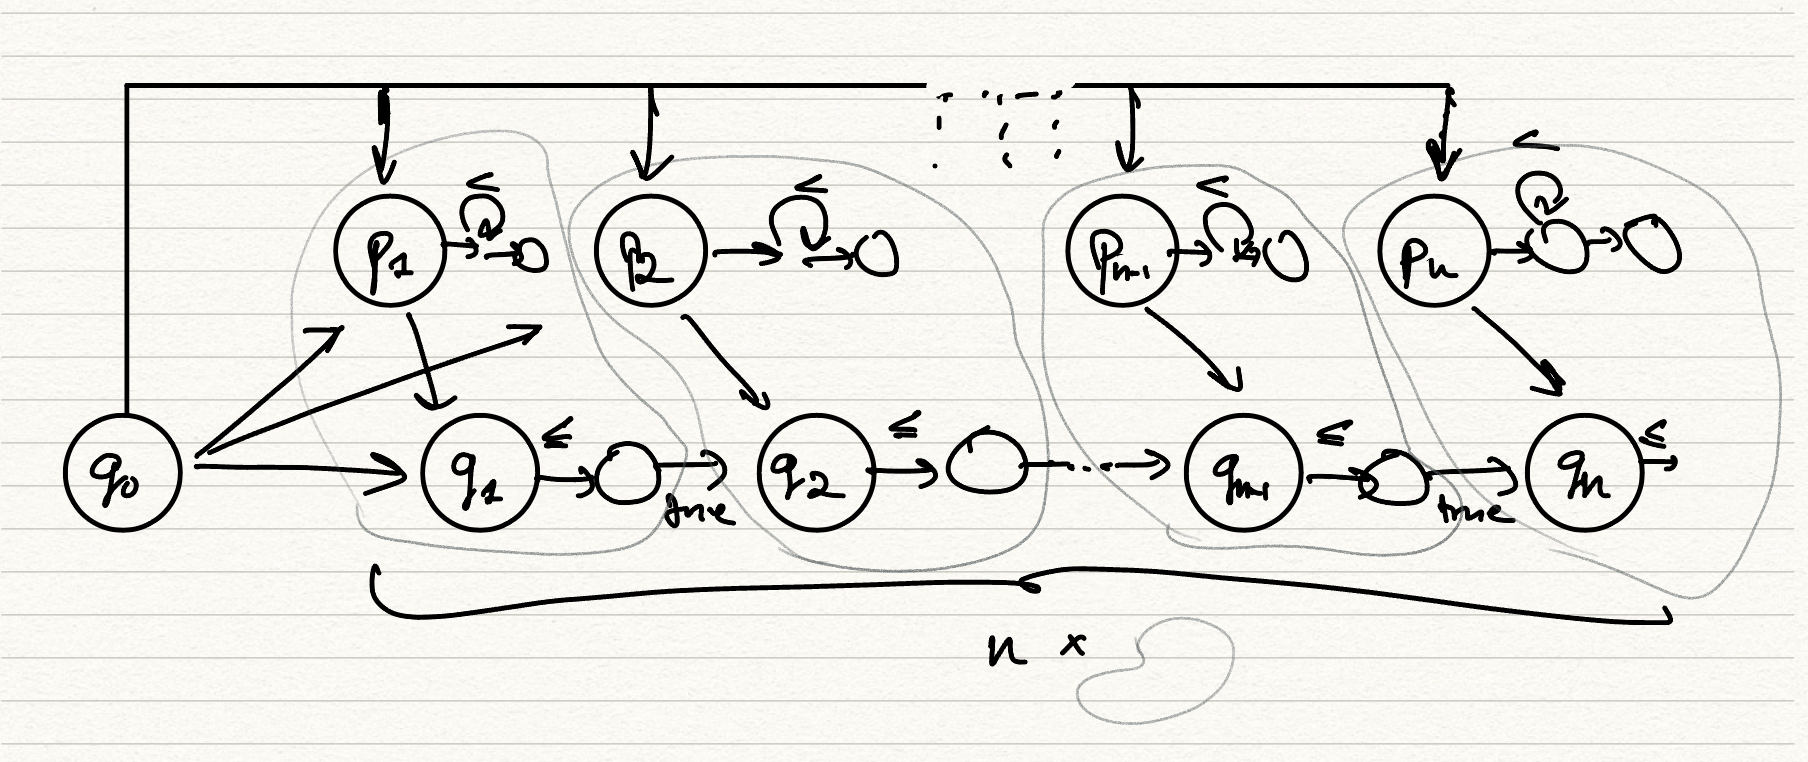
\includegraphics[width=0.8 \textwidth]{figures/naive_vs_relaxed.jpeg}
        \caption{An illustration of $\mathcal{A}_n$}
    \end{figure}

    Let the states $p_i$ have only one $\geq$ transition, and let the states $q_i$ have $m$ transitions with guard $\geq$ and no $<$ transitions. 

    All other transitions not shown in this diagram are to a designated terminal state, which is also not shown as they are not relevant to the proof. Let us denote the shift assigned to a segment $s$ by $\gamma_s$.

    Any naive shift-coupling proof of privacy assigns a shift of $\gamma_{p_i} = 1$ since $p_i$ has an $L$-cycle. Since $p_i \hookrightarrow q_i$, we have that $\gamma_{p_i} \leq \gamma_{q_i}$, which forces $\gamma_{q_i} = 1$. Let $q_0$ be the initial segment with some coupling cost $c_0$. Let $c_1$ bound the cost of the segment $p_i$ if we choose $\gamma_{p_i} = 1$. 
    
    The cost of constructing the naive shift-coupling proof of privacy is then the maximum cost over all segments, which is $q_0 \to p_1 \to q_1 \to \dots \to q_n$. This has cost at least $c_0 + c_1 + n \cdot (2 + 2m)$, or 

    \[\text{ naive cost } \geq c_0 + c_1 + 2n + 2mn\]

    However, the cost of the relaxed shift-coupling proof of privacy is at most $c_0 + c_1 + 2 + 2m + 2n$, since only one of the $q_i$ segments would have a shift of $1$ for any given sequence of segments. This is because paths traverse through at most one $p_i$, and the shifts on $q_i$ do not constrain each other. 

    \[\text{ relaxed cost } \leq c_0 + c_1 + 2 + 2m + 2n\]

    If we let $m = n$, then we get that the naive cost is in $\Omega(n^2)$ while the relaxed cost is in $O(n)$.

\end{proof}


\section{Is the tight shift-coupling proof also a tight coupling proof?}
\textbf{Last Updated: Wednesday, June 28th, 2023}

The relevant definitions and lemmata for proofs in this section are in the appendix. It is also assumed, for now, that all transition outputs are in the output alphabet. 

\subsection{Conjecture: $S^L$ is tight when there is an $L$-cycle}

\begin{conjecture} ($S^L$ is tight for segments with $L$-cycles)
    \label
    Consider a segment $s \in seg(\mathcal{A})$ corresponding to the sequence of states $q_0 \to q_1 \to \dots \to q_m$. If $s$ contains an $L$-cycle, then the L-cost of the segment gives a tight upper bound on the privacy loss of the segment. That is, \[\loss(s) =  \exp\left(2 \epsilon_0 + \sum_{i > 0: guard(a_i) = \insamplegeqx} 2\epsilon_i \right)\]

    given that state $q_i$ draws from the distribution $Lap(0, 1/\epsilon_i)$ to noise \insample.
\end{conjecture}

\begin{proof}
    Note: the proof of this conjecture can be reduced to showing Lemma \ref{lemma:sl_asymptotic}.
    We will prove the result for when $\epsilon_i = \epsilon$ for all $i \geq 0$. The proof for the general case goes through in the same fashion. Let $f, F$ be the probability density function and cumulative distribution function of a random variable $X$ with $X \sim Lap(0, 1/\epsilon)$ as defined in the appendix. 

    Since $s$ has an L-cycle, there exists a sequence of paths $\rho_i$ for $i \in \N$ each with $l_i$ number of L-transitions such that $\lim_{i \to \infty} l_i = \infty$. Let $m$ be the number of $G$-transitions in $\rho_i$. We will assume that this number is the same across all $\rho_i$.\footnote{Otherwise, $s$ has a G-cycle, and $\mathcal{A}$ is not differentially private. The privacy loss through $s$ is $\infty$, which matches the $L$-cost.}
    
    For each $\rho_i$, construct the adjacent pair of inputs $X_i, X_i'$ as follows. Let $X_i[j] = 0$ for all $j \in \{1, \dots, |\rho_i|\}$, where $|\rho_i|$ is the number of transitions in $\rho$. Define $X_i[j]$ as follows:

    \[X_i[j] = \begin{cases}
        1 & \text{if } \rho_i[j] \to \rho_i[j + 1] \text{ is an assignment transition or has guard \insamplegeqx} \\
        -1 & \text{otherwise, in which case } \rho_i[j] \to \rho_i[j + 1] \text{ has guard \insampleltx}\\
    \end{cases}\]

    Let $\tilde{a_j}$ be the random variable representing the value of $\insample$ before the $j$th transition in $\rho$ on input $X_i$. Let $\tilde{b_j}$ be the random variable representing the value of $\insample$ before the $j$th transition in $\rho$ on input $X_i'$. Further, let $\Gamma_L = \{j : \rho_i[j] \to \rho_i[j + 1] \text{ has guard } \insampleltx\}$, and $\Gamma_G = \{j : \rho_i[j] \to \rho_i[j + 1] \text{ has guard } \insamplegeqx\}$. 
    
    Notice that $\tilde{a_j} = \tilde{b_j} + 1$ for $j \in \Gamma_L$, and $\tilde{a_j} + 1 = \tilde{b_j}$ for $j \in \{0\} \cup \Gamma_G$. Since $\tilde{a_j}$ is distributed as $Lap(X_i[j], 1/\epsilon)$, we can write its probability density function as $f(x - X_i[j])$, and its cumulative distribution function as $F(x - X_i[j])$. A similar statement holds for $\tilde{b_j}$.
    
    We may now compute and compare $Pr(\rho_i | X_i')$ and $\Pr(\rho_i | X_i)$ as follows.

    \begin{align*}
        \Pr(\rho_i | X_i') &= \int_{-\infty}^\infty \Pr(\tilde{b_0} = x) \prod_{j \in \Gamma_L} \Pr(\tilde{b_j} < x) \prod_{j \in \Gamma_G} \Pr(\tilde{b_j} \geq x) \dif x\\
        &= \int_{-\infty}^\infty \Pr(\tilde{b_0} = x) \prod_{j \in \Gamma_L} \Pr(\tilde{b_j} < x) \prod_{j \in \Gamma_G} \Pr(\tilde{b_j} \geq x) \dif x\\
        &= \int_{-\infty}^\infty f_\epsilon(x - X_i[0]) \prod_{j \in \Gamma_L} F_\epsilon(x - X_i[j]) \prod_{j \in \Gamma_G} (1 - F_\epsilon(x - X_i[j])) \dif x\\
        &= \int_{-\infty}^\infty f(x - 1) F(x + 1)^{\ell_i}  (1 - F(x - 1))^m \\
        &= \int_{-\infty}^\infty f(x) F(x + 2)^{\ell_i}  (1 - F(x))^m \\
        &= \exp(2\epsilon (m + 1) )\left(\int_{(-\infty, -2) \cup (2, \infty)} f(x) F(x)^{\ell_i}  (1 - F(x))^m \dif x + g(\ell_i) \int_{-2}^2 f(x) F(x + 2)^{\ell_i}  (1 - F(x))^m\right)
    \end{align*}

    with $g(\ell_i) \to 1$ as $\ell_i \to \infty$. As we take $\ell_i \to \infty$, we see that 

    \begin{align*}
        h(\ell_i) := \frac{\left(\int_{(-\infty, -2) \cup (2, \infty)} f(x) F(x)^{\ell_i}  (1 - F(x))^m \dif x + g(\ell_i) \int_{-2}^2 f(x) F(x + 2)^{\ell_i}  (1 - F(x))^m\right)}{\Pr(\rho_i | X_i)} \to 1
    \end{align*}

    and so as we take the supremum over $\rho_i$ below, we get: 

    \begin{align*}
        \loss(s) \geq \sup_{\rho_i} \frac{\Pr(\rho_i | X_i')}{\Pr(\rho_i | X_i)} &= \exp(2\epsilon(m + 1)) \sup_{\rho_i} \left\{ h(l_i) \right\}\\
        &= \exp(2\epsilon(m + 1))
    \end{align*}

    We know that $S^L$ is tight, and gives the bound $\exp(2\epsilon(m + 1))$. Thus, we have shown that $\loss(s) = \exp(2\epsilon(m + 1))$, as desired.
\end{proof}

\subsection{Investigating costs of alternative coupling strategies}

\begin{definition}
    $S^J$ is a coupling strategy in which we do not couple the noised threshold, but couple the results of all other transitions with twice the cost. 
\end{definition}

\begin{theorem}
    Let $s = q_0 \to \dots \to q_m$ be a segment with only L-transitions. If $S^J$ is the least-cost coupling strategy on $s$, then it provides a tight bound on $\loss(s)$ given by \[\loss(s) = \sum_{i = 1}^{m} 2\epsilon_i\]
\end{theorem}

\begin{proof}
    Follows from some algebra.

    \begin{figure}[H]
        \centering
        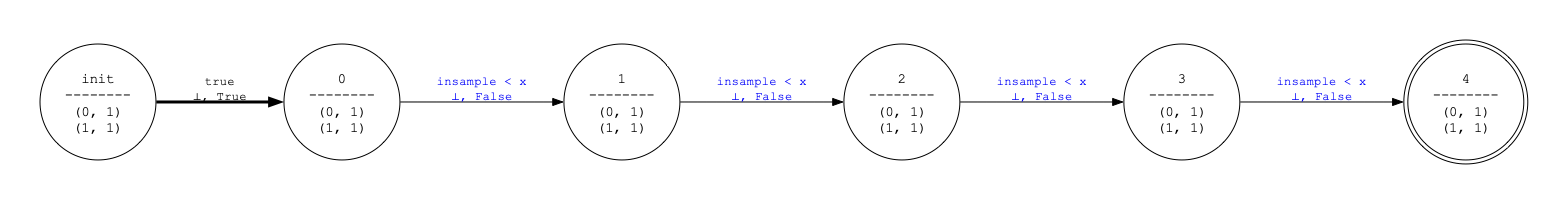
\includegraphics[width=0.9\textwidth]{figures/only_l_transitions.png}
        \caption{A segment $s$ with only L-transitions.}
        \label{fig:segment_j}
    \end{figure}

    \begin{figure}[H]
        \centering
        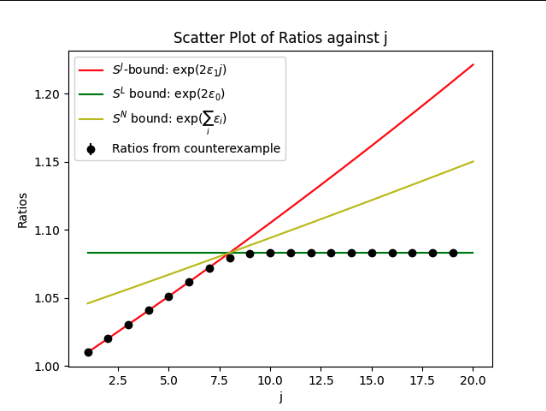
\includegraphics[width=0.5\textwidth]{figures/only_l_transitions_plot.png}
        \caption{}
        \label{fig:segment_j_coupling}
    \end{figure}
\end{proof}

\begin{conjecture}
    For segments which contain only $L$-transitions and for which the $J$-cost exceeds the $L$-cost, $S^L$ is tight.
\end{conjecture}

\begin{proof}
    I think this is true from the graph above, but I need to prove it.

    Note June 28 2023: I think this is not true for segments that contain both $L$-transitions and $G$-transitions.
\end{proof}

\subsection*{Lemmata}

\subsubsection*{Properties of $f_\epsilon$ and $F_\epsilon$}

\begin{lemma} 
    \label{lemma:F_equality_neg}
    For $x \leq 0$, we have 
    \[F_\epsilon(x) = \exp(2\epsilon)F_\epsilon(x - 2)\]
    and equivalently for $x \leq -2$, we have 
    \[F_\epsilon(x + 2) = \exp(2\epsilon)F_\epsilon(x)\]
\end{lemma}

\begin{lemma}
    \label{lemma:F_equality_pos}
    For $x \geq 0$, we have \[1 - F_{\epsilon}(x) = \exp(2\epsilon) (1 - F_\epsilon(x + 2))\]
\end{lemma}

\begin{lemma}
    \label{lemma:f_equality}
    For $x \geq 0$, we have
    \[f_\epsilon(x) = \exp(2\epsilon) f_\epsilon(x + 2) \]
\end{lemma}

\subsubsection*{For the proof of Theorem 1}
\begin{lemma} 
    \label{lemma:sl_tight_minus_infty} 
    \[\int_{-\infty}^{-2} f_{\epsilon}(x) F_{\epsilon}(x + 2)^\ell (1 - F_{\epsilon}(x))^m \dif x = \exp(2 \epsilon \ell) \int_{-\infty}^{-2} f_{\epsilon}(x) F_{\epsilon}(x)^\ell (1 - F_{\epsilon}(x))^m \dif x\]
\end{lemma}

\begin{proof}
    From Lemma \ref{lemma:F_equality_neg}, we have that 

    \begin{align*}
        \int_{-\infty}^{-2} f_{\epsilon}(x) F_{\epsilon}(x + 2)^\ell (1 - F_{\epsilon}(x))^m \dif x &= \int_{-\infty}^{-2} f_{\epsilon}(x) (\exp(2\epsilon) F_{\epsilon}(x))^\ell (1 - F_{\epsilon}(x))^m \dif x \\
        &= \exp(2\epsilon \ell) \int_{-\infty}^{-2} f_{\epsilon}(x) F_{\epsilon}(x)^\ell (1 - F_{\epsilon}(x))^m \dif x
    \end{align*}
\end{proof}

\begin{lemma}
    \label{lemma:sl_tight_plus_infty}
    \[\int_{0}^{\infty} f_{\epsilon}(x) F_{\epsilon}(x + 2)^\ell (1 - F_{\epsilon}(x))^m \dif x = \exp(2 \epsilon m) \int_{2}^{\infty} f_{\epsilon}(x) F_{\epsilon}(x)^\ell (1 - F_{\epsilon}(x))^m \dif x\]
\end{lemma}

\begin{proof}
    From Lemma \ref{lemma:F_equality_pos} and \ref{lemma:f_equality}, we have that

    \begin{align*}
        \int_{0}^{\infty} f_{\epsilon}(x) F_{\epsilon}(x + 2)^\ell (1 - F_{\epsilon}(x))^m \dif x &= \int_{0}^{\infty} \exp(2\epsilon)f_{\epsilon}(x + 2) F_{\epsilon}(x + 2)^\ell (\exp(2\epsilon)(1 - F_{\epsilon}(x + 2)))^m \dif x \\
        &= \exp(2\epsilon m) \int_{0}^{\infty} f_{\epsilon}(x + 2) F_{\epsilon}(x + 2)^\ell (1 - F_{\epsilon}(x + 2))^m \dif x\\
        &= \exp(2\epsilon (m + 1)) \int_{2}^{\infty} f_{\epsilon}(x) F_{\epsilon}(x)^\ell (1 - F_{\epsilon}(x))^m \dif x
    \end{align*}
\end{proof}

\begin{lemma}
    \label{lemma:sl_asymptotic}
    There exists a function $g: \N \to \mathbb{R}$ such that
    \label{lemma:sl_tight_minus_2}
    \[\int_{-2}^{0} f_{\epsilon}(x) F_{\epsilon}(x + 2)^\ell (1 - F_{\epsilon}(x))^m \dif x = g(\ell) \exp(2 \epsilon (m + 1)) \int_{-2}^{2} f_{\epsilon}(x) F_{\epsilon}(x)^\ell (1 - F_{\epsilon}(x))^m \dif x\]
    with $g(\ell) \to 1$ as $\ell \to \infty$.
\end{lemma}

\begin{proof}
    I'm not sure yet how to prove this, although I strongly suspect that the $(m + 1)$ term comes from the fact that $f_{\epsilon}(x)$ is the derivative of $-(1 - F_{\epsilon}(x))$, and it is taken to the $m$th power. Its integral should behave like a polynomial of degree $m + 1$ evaluated at $2$, which corresponds to $\exp(2\epsilon(m + 1))$. 
\end{proof}


\end{document}